
\documentclass[12pt]{report}
\author{Javad Ibrahimli}


% Inputs the Document Packages
\input{_Packages}

% Controls how many subsections the document can take
%  and how many of those will get put into the contents pages.
\setcounter{secnumdepth}{3}
\setcounter{tocdepth}{3}

% Line Spacing
\setstretch{1.5}


% Places a dot after Chapter/Section/Subsection number in Table of Contents
\renewcommand{\cftchapaftersnum}{.}
\renewcommand{\cftsecaftersnum}{.}
\renewcommand{\cftsubsecaftersnum}{.}

%  Customize Dot spacing in Table of Contents/List of Figures/Tables
\renewcommand{\cftdotsep}{0.3}


% Line Break Properties
\tolerance=1
\emergencystretch=\maxdimen
\hyphenpenalty=10000
\hbadness=10000


% Formatting Table of Contents/Lists titles
\renewcommand{\contentsname}{\bfseries\LARGE{CONTENTS}}
\renewcommand{\listfigurename}{\bfseries\LARGE{LIST OF FIGURES}}

% Signature Line for the declaration
\newbox\namebox
\newdimen\signboxdim

\def\signature#1{%
    \setbox\namebox=\hbox{#1}
    \signboxdim=\dimexpr(\wd\namebox+3cm)
    \parbox[t]{\signboxdim}{%
        \centering
            \hrulefill\\    % for a line
            #1
        \par}%
    }

% Title Formatting customization
\titleformat{\chapter}{\normalfont\bfseries\LARGE}{\thechapter.}{1em}{\MakeUppercase}

\titleformat{\section}{\normalfont\bfseries\large}{\thesection.}{1em}{\MakeUppercase}
\titlespacing*{\section} {0pt} {0pt} {15pt} % left, before, after

\titleformat{\subsection}{\normalfont\bfseries\large}{\thesubsection.}{1em}{}
\titlespacing*{\subsection} {0pt} {10pt} {10pt}

\titleformat{\subsubsection}{\normalfont\bfseries\large}{\thesubsubsection.}{1em}{}
\titlespacing*{\subsubsection} {0pt} {10pt} {10pt}


% HEADER AND FOOTER
\pagestyle{fancy}  % Set Page Style (Header and Footer Style)
\fancyhf{}  % Clears the header and footer (from the default info)

% Header
\renewcommand{\headrulewidth}{0pt}  % Removes the default Horizontal Line in Header
% Optional Headers
%\fancyhead[L]{}
%\fancyhead[R]{2022/2023}

% Footer
\fancyfoot[C]{\thepage} % Page Number

% Change figure numbering per section
\numberwithin{figure}{chapter}

%Acronym entries
\makeglossaries
\newacronym{US}{US}{Ultrasound}



%  -------------------------------------------------
%  --------- The document starts from here --------- 
%  -------------------------------------------------

\begin{document}


% ------------------  TITLE PAGE -------------------

\begin{titlepage}
{\color{purple}
\begin{center}
    
    % UCL IMAGE
    \vspace*{-2.5cm}
    \makebox[\textwidth]{\includegraphics[scale=0.6]{Images/logo_800anni.png}}
    
    \vspace{2.3cm}
    

    \vspace{1cm}
    {\relscale{1.3}\textbf{NUMERICAL METHODS FOR DIFFERENTIAL EQUATIONS \\}}
    \vspace{0.3cm}
    {\relscale{1.35}\textbf{INP5070378\\}}
    \vspace{2.4cm}
    
    {\relscale{2.00}{HOMEWORK 3}}\\
    %\vspace{0.1cm}
    By\\
    %\vspace{0.1cm}
    Alessandro Crotti \\ 
    \vspace{0.9cm}
    {\begin{singlespace}Course given by:\\\end{singlespace}}
    {\begin{singlespace}Luca Bergamaschi\\
    Andrea Franceschini\\\end{singlespace}}


\end{center}
{\raggedleft\vfill{\begin{singlespace}
     Department of Civil, Construction and Environmental engineering\\
\end{singlespace}
 Mathematical Engineering\\
 \begin{singlespace}
 % Date of submission: \today\\

 
 \end{singlespace} 
 
}\par
}
}
\end{titlepage}




% ------------------  TABLE OF CONTENTS --------------------
\tableofcontents 






% -------------------  INTRODUCTION  ---------------------
\chapter{Problem}
In this Homework we have to solve the following Heat Equation \eqref{eq: Heat_equation} with the Finite Element Method (FEM). The domain is $\Omega \subset \mathbb{R}^2$ and it can be seen in Fig, \ref{fig: domain}.

\begin{equation}\label{eq:Heat_equation}
\begin{aligned}
    \text{Given} \quad &f(\mathbf{x},t) : \Omega \times \mathbb{T} \longrightarrow \mathbb{R}, \ d_1(\mathbf{x},t):\Gamma_{D,1} \times \mathbb{T} \longrightarrow \mathbb{R},\\
    &d_2(\mathbf{x},t):\Gamma_{D,2} \times \mathbb{T} \longrightarrow \mathbb{R}, \ q(\mathbf{x},t):\Gamma_{N} \times \mathbb{T} \longrightarrow \mathbb{R}, \\
    &u_0(\mathbf{x}): \overline{\Omega} \longrightarrow \mathbb{R}.\\
    \text{find} \quad &u(\mathbf{x},t) \in \overline{\Omega} \times \mathbb{T} \ \text{such that:}\\
    &\begin{cases}
        \begin{aligned}
            \frac{\partial u(\mathbf{x},t)}{\partial t} &- \frac{\partial^2u(\mathbf{x},t)}{\partial x^2}-\frac{\partial^2u(\mathbf{x},t)}{\partial^2y}=f(\mathbf{x},t) & \text{in} \quad &\Omega \times \mathbb{T} \\
            
            u(\mathbf{x},t) &=d_1(\mathbf{x},t) & \text{on} \quad &\Gamma_{D,1} \times \mathbb{T} \\
            
            u(\mathbf{x},t) &=d_2(\mathbf{x},t) & \text{on} \quad &\Gamma_{D,2} \times \mathbb{T} \\
            
            \frac{\partial u(\mathbf{x},t)}{\partial \mathbf{n}} &=1(\mathbf{x},t) & \text{on} \quad &\Gamma_{N} \times \mathbb{T} \\
            
            u(\mathbf{x},0) &= u_0(\mathbf{x}) & \text{in} \quad &\overline{\Omega} 
        \end{aligned}
    \end{cases}
\end{aligned}
\end{equation}
The problem is Homogeneous that means $f(\mathbf{x},t)=0$. The Dirichlet boundary condition for $\Gamma_D=\Gamma_{D,1}\cup \Gamma_{D,2}$ imposed $d_1(\mathbf{x},t)=0$ and $d_2(\mathbf{x},t)$ linear up to $1$, reached at $t=t_max/2$, then equal to $1$. The Neumann boundary condition on $\Gamma_N$ is given by the function $q(\mathbf{x},t)=0$ and the initial solution $u_0(\mathbf{x},t)=0$. The final time is $t_max=10$.
We have to solve the initial boundary value problem \eqref{eq:Heat_equation} with FEM using triangular elements and linear basis functions. 

\begin{figure}[h]
    \centering
    \includegraphics[width=0.5\textwidth]{Images/problem/domain.png}
        \caption{Domain $\Omega$ with boundary and points of interest}
        \label{fig: domain}
\end{figure}


 % Section/Chapter entries can be done in the Main.tex file or in a  
                       % separate tex file for longer and more complex documents


% -------------------  MATERIALS AND METHODS  ---------------------
\chapter{Code}
In this Homework we have to solve the following Heat Equation \eqref{eq: Heat_equation} with the Finite Element Method (FEM). The domain is $\Omega \subset \mathbb{R}^2$ and it can be seen in Fig, \ref{fig: domain}.

\begin{equation}\label{eq:Heat_equation}
\begin{aligned}
    \text{Given} \quad &f(\mathbf{x},t) : \Omega \times \mathbb{T} \longrightarrow \mathbb{R}, \ d_1(\mathbf{x},t):\Gamma_{D,1} \times \mathbb{T} \longrightarrow \mathbb{R},\\
    &d_2(\mathbf{x},t):\Gamma_{D,2} \times \mathbb{T} \longrightarrow \mathbb{R}, \ q(\mathbf{x},t):\Gamma_{N} \times \mathbb{T} \longrightarrow \mathbb{R}, \\
    &u_0(\mathbf{x}): \overline{\Omega} \longrightarrow \mathbb{R}.\\
    \text{find} \quad &u(\mathbf{x},t) \in \overline{\Omega} \times \mathbb{T} \ \text{such that:}\\
    &\begin{cases}
        \begin{aligned}
            \frac{\partial u(\mathbf{x},t)}{\partial t} &- \frac{\partial^2u(\mathbf{x},t)}{\partial x^2}-\frac{\partial^2u(\mathbf{x},t)}{\partial^2y}=f(\mathbf{x},t) & \text{in} \quad &\Omega \times \mathbb{T} \\
            
            u(\mathbf{x},t) &=d_1(\mathbf{x},t) & \text{on} \quad &\Gamma_{D,1} \times \mathbb{T} \\
            
            u(\mathbf{x},t) &=d_2(\mathbf{x},t) & \text{on} \quad &\Gamma_{D,2} \times \mathbb{T} \\
            
            \frac{\partial u(\mathbf{x},t)}{\partial \mathbf{n}} &=1(\mathbf{x},t) & \text{on} \quad &\Gamma_{N} \times \mathbb{T} \\
            
            u(\mathbf{x},0) &= u_0(\mathbf{x}) & \text{in} \quad &\overline{\Omega} 
        \end{aligned}
    \end{cases}
\end{aligned}
\end{equation}
The problem is Homogeneous that means $f(\mathbf{x},t)=0$. The Dirichlet boundary condition for $\Gamma_D=\Gamma_{D,1}\cup \Gamma_{D,2}$ imposed $d_1(\mathbf{x},t)=0$ and $d_2(\mathbf{x},t)$ linear up to $1$, reached at $t=t_max/2$, then equal to $1$. The Neumann boundary condition on $\Gamma_N$ is given by the function $q(\mathbf{x},t)=0$ and the initial solution $u_0(\mathbf{x},t)=0$. The final time is $t_max=10$.
We have to solve the initial boundary value problem \eqref{eq:Heat_equation} with FEM using triangular elements and linear basis functions. 

\begin{figure}[h]
    \centering
    \includegraphics[width=0.5\textwidth]{Images/problem/domain.png}
        \caption{Domain $\Omega$ with boundary and points of interest}
        \label{fig: domain}
\end{figure}


 % Section/Chapter entries can be done in the Main.tex file or in a  
                       % separate tex file for longer and more complex documents


% -------------------  MATERIALS AND METHODS  ---------------------
\chapter{Results}
In this section the results will be reported, highlighting the difference between the different meshes. 

The solutions are computed with PCG method using Jacobi as precondition and with the incomplete Cholesky factorization. The last one solution is displayed in Fig. \ref{fig: stationary_solution}.

In Tab. \ref{tab: data_point} is displayed the solution at different times for points $P_1$, $P_2$ and $P_3$.

In Fig. \ref{fig: boundary_solution} the solutions along the boundary are displayed for different meshes at times $2.5$, $5.0$, $7.5$ and $10.0$.

In Fig. \ref{fig: track point for all time} the solutions for the three points for all the whole time are displayed. Each figure indicates differents meshes.

The value of the ratio $\mathbf{r}$ and the error $\mathbf{\varepsilon}$ are displayed in Tab. \ref{tab: table_R_error}. 
The ratio $\mathbf{r}$ helps assess how the error changes relative to the change in the mesh refinement level. A value of $\mathbf{r}$ close to 1 suggests that the error is changing proportionally to the change in mesh refinement level, indicating a balanced refinement. Deviations from 1 may indicate over-refinement or under-refinement, providing insights into the effectiveness of the mesh and the convergence behavior of the numerical solution.
The ratio are computed as follow $$\mathbf{r}=\frac{\varepsilon_{k-1}}{\varepsilon_k} ( \frac{h_k}{h_{k-1}})^2$$
The vector $\mathbf{h}$ contains the maximum Euclidean distance between any two vertices in the mesh for each iteration (so for each mesh). It can be interpreted as a measure of the characteristic size or diameter of the mesh.
The vector $\mathbf{\varepsilon}$ represents the error norms comparing the solution obtained with the real solution.
$$\varepsilon \simeq \sqrt{ \sum_{i=1}^{n}[(u_i-u(\mathbf{x_i},\mathbf{y_i}))^2 \frac{\Sigma_e \Delta_e}{3}]}$$
The parameter $\Delta_e$ is computed as explained in the previous chapter.

In Fig. \ref{fig: Residual normal cholensky} and Fig. \ref{fig: Residual normal jacobi} are dispalyed the residual norma in semi logaritmic scale for the Cholensky and Jacobi preconditioner respectively.

%---------------------------------------SOLUTION---------------------------------------------------

\begin{figure}[htbp]
    \centering
    \begin{subfigure}{0.45\textwidth}
        \centering
        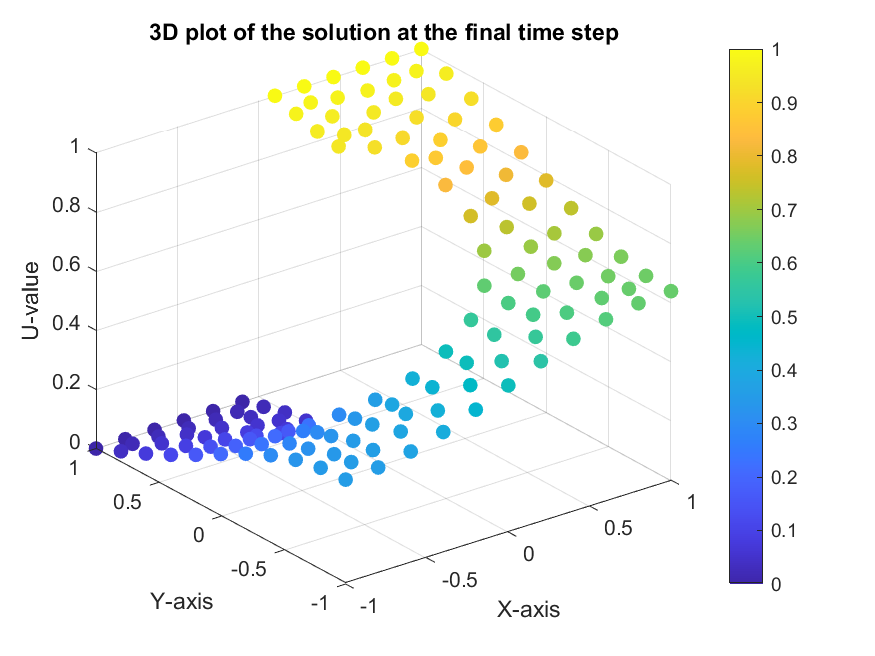
\includegraphics[width=\linewidth,trim=0mm 0mm 0mm 7.5mm, clip]{Images/mesh0/u_chol_mesh0.png}
        \caption{mesh0}
    \end{subfigure}
    \hfill
    \begin{subfigure}{0.45\textwidth}
        \centering
        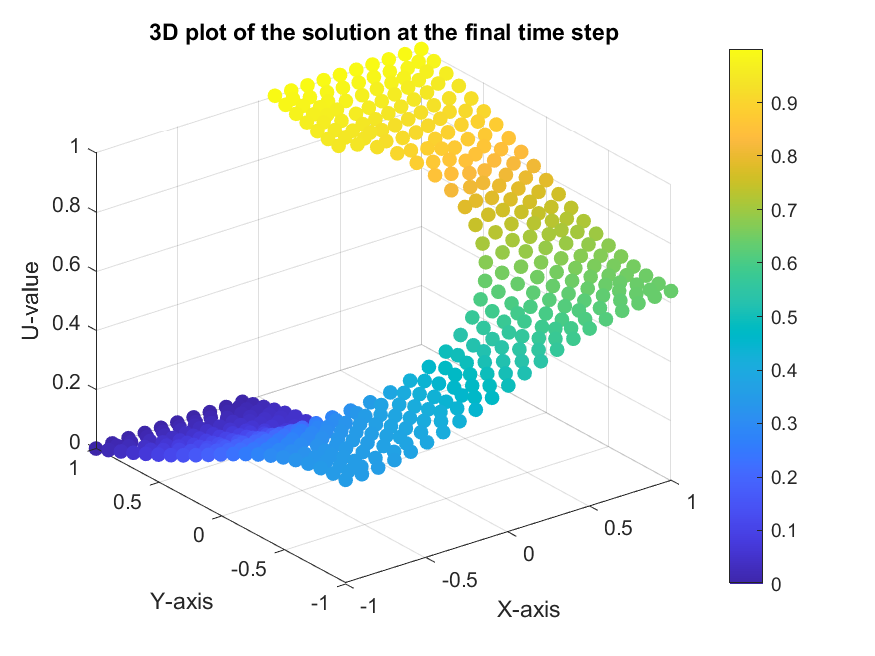
\includegraphics[width=\linewidth,trim=0mm 0mm 0mm 7.5mm, clip]{Images/mesh1/u_chol_mesh1.png}
        \caption{mesh1}
    \end{subfigure}
    \hfill
    \begin{subfigure}{0.45\textwidth}
        \centering
        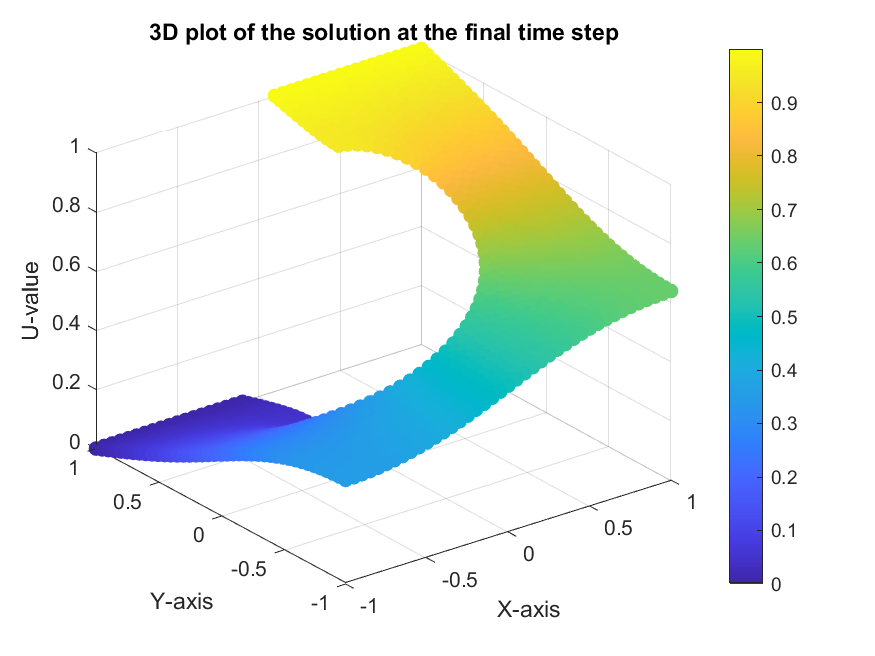
\includegraphics[width=\linewidth,trim=0mm 0mm 0mm 7.5mm, clip]{Images/mesh2/u_chol_mesh2.png}
        \caption{mesh2}
    \end{subfigure}

    \vspace{1em} % Spacing between rows

    \begin{subfigure}{0.45\textwidth}
        \centering
        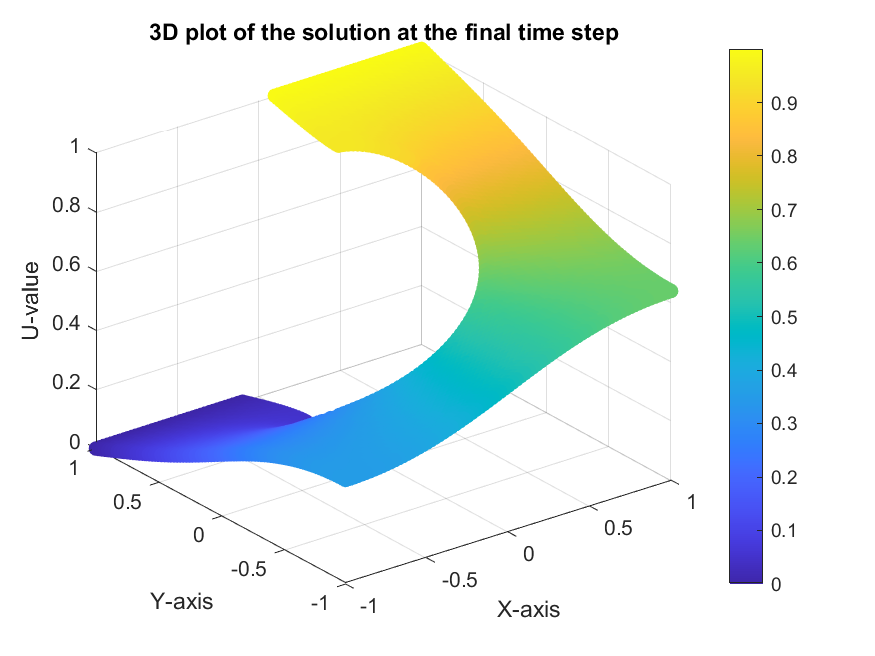
\includegraphics[width=\linewidth,trim=0mm 0mm 0mm 7.5mm, clip]{Images/mesh3/u_chol_mesh3.png}
        \caption{mesh3}
    \end{subfigure}
    \hfill
    \begin{subfigure}{0.45\textwidth}
        \centering
        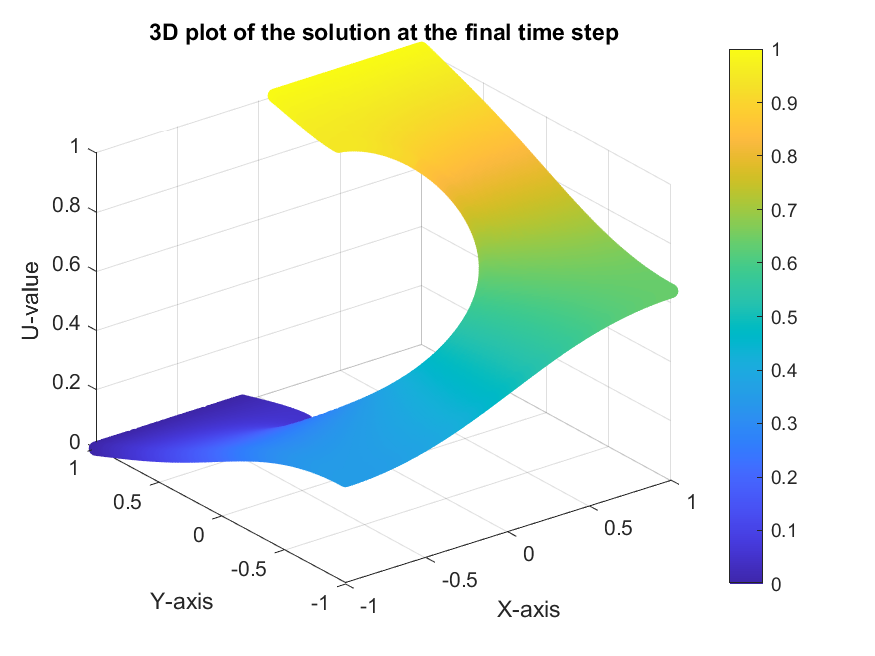
\includegraphics[width=\linewidth,trim=0mm 0mm 0mm 7.5mm, clip]{Images/mesh4/u_chol_mesh4.png}
        \caption{mesh4}
    \end{subfigure}

    \caption{Stationary solution on different meshes}
    \label{fig: stationary_solution}
\end{figure}

%--------------------------------TRACE----------------------------------------------------
 
\begin{figure}[htbp]
    \centering
    \begin{subfigure}{0.45\textwidth}
        \centering
        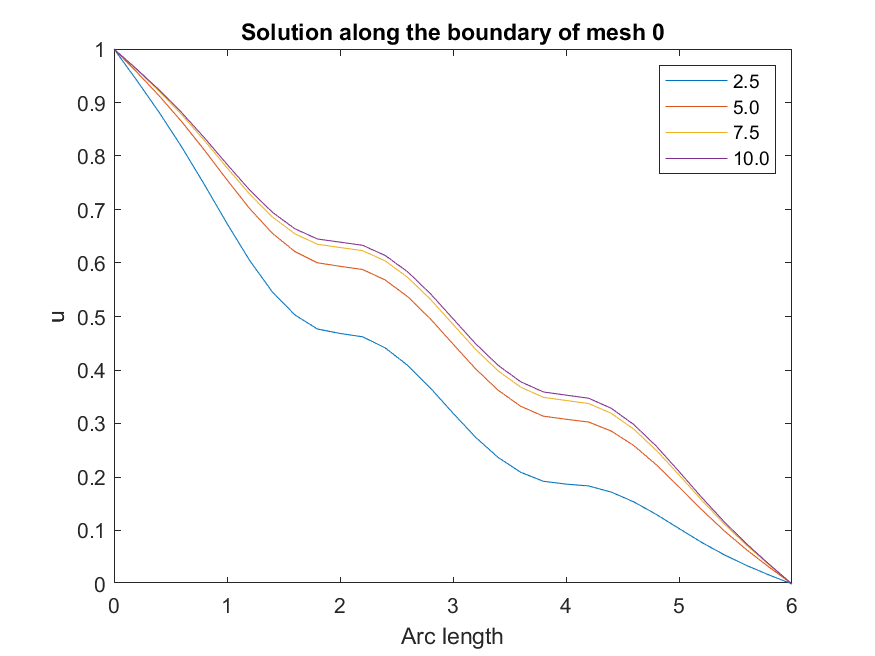
\includegraphics[width=\linewidth,trim=0mm 0mm 0mm 7.5mm, clip]{Images/mesh0/trace_u_chol_mesh0.png}
        \caption{mesh0}
    \end{subfigure}
    \hfill
    \begin{subfigure}{0.45\textwidth}
        \centering
        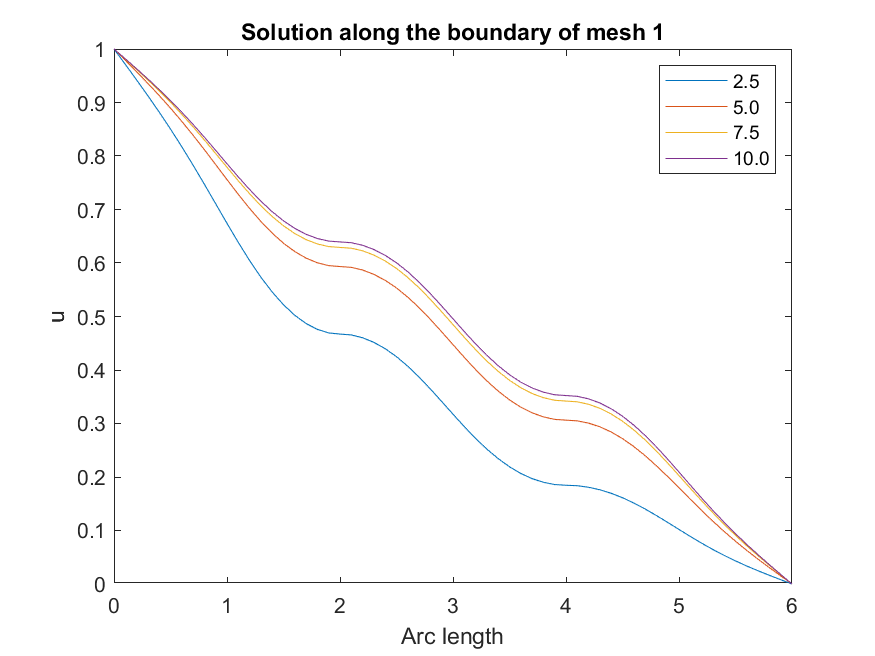
\includegraphics[width=\linewidth,trim=0mm 0mm 0mm 7.5mm, clip]{Images/mesh1/trace_u_chol_mesh1.png}
        \caption{mesh1}
    \end{subfigure}
    \hfill
    \begin{subfigure}{0.45\textwidth}
        \centering
        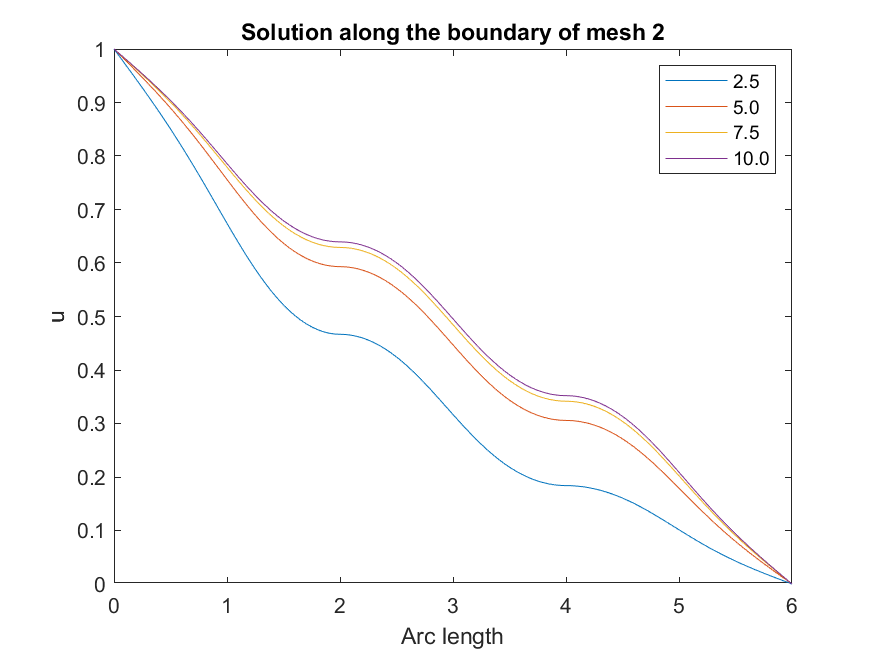
\includegraphics[width=\linewidth,trim=0mm 0mm 0mm 7.5mm, clip]{Images/mesh2/trace_u_chol_mesh2.png}
        \caption{mesh2}
    \end{subfigure}

    \vspace{1em} % Spacing between rows

    \begin{subfigure}{0.45\textwidth}
        \centering
        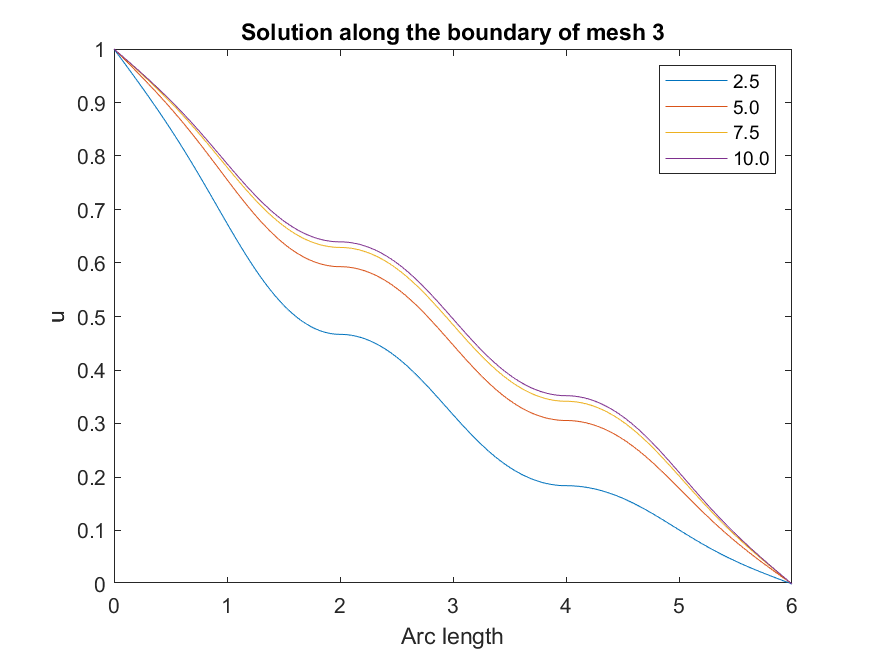
\includegraphics[width=\linewidth,trim=0mm 0mm 0mm 7.5mm, clip]{Images/mesh3/trace_u_chol_mesh3.png}
        \caption{mesh3}
    \end{subfigure}
    \hfill
    \begin{subfigure}{0.45\textwidth}
        \centering
        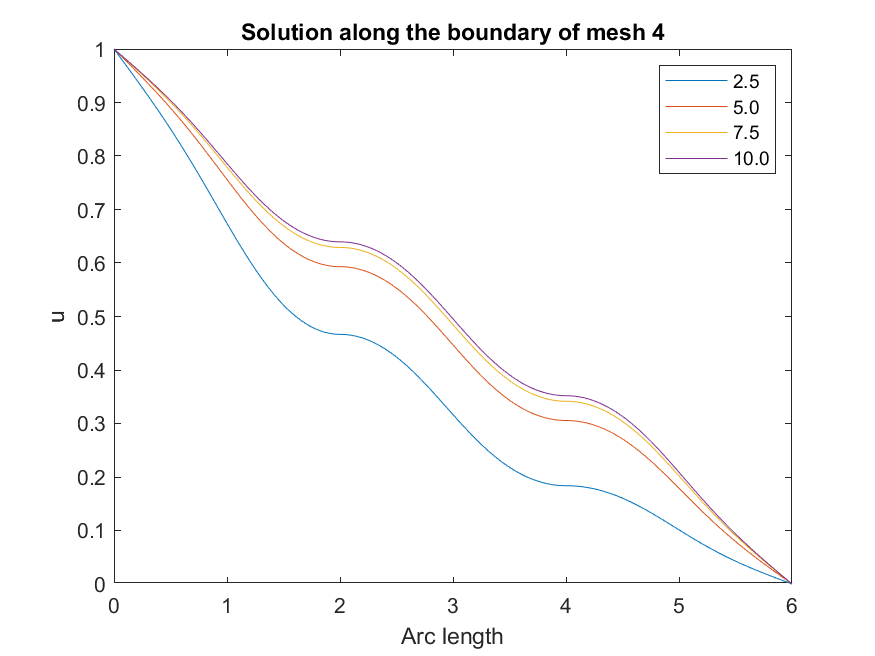
\includegraphics[width=\linewidth,trim=0mm 0mm 0mm 7.5mm, clip]{Images/mesh4/trace_u_chol_mesh4.png}
        \caption{mesh4}
    \end{subfigure}

    \caption{Solution along the boundary on different meshes at three different times}
    \label{fig: boundary_solution}
\end{figure}

%------------------------------TRACK-------------------------------------------------
 
\begin{figure}[htbp]
    \centering
    \begin{subfigure}{0.45\textwidth}
        \centering
        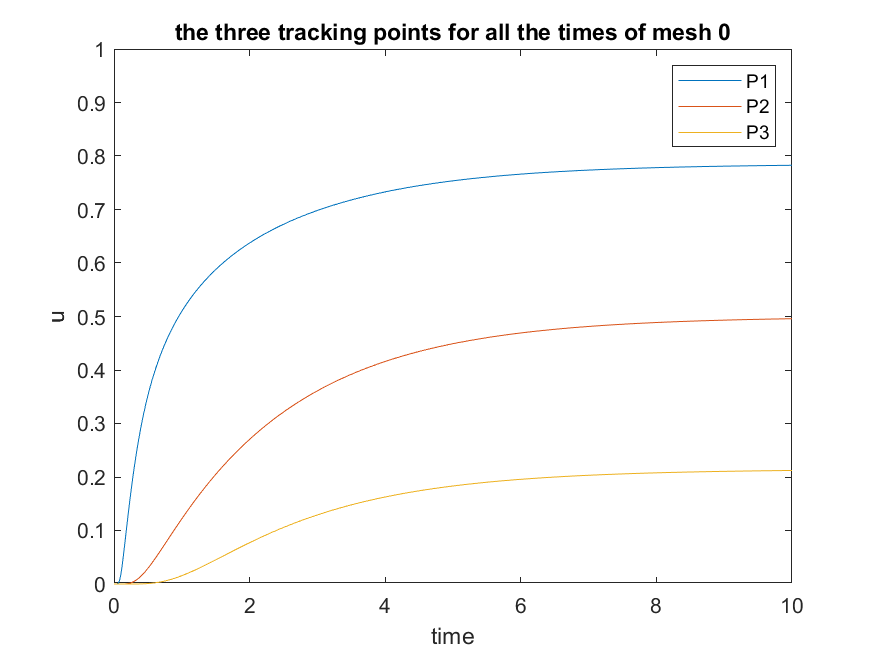
\includegraphics[width=\linewidth,trim=0mm 0mm 0mm 7.5mm, clip]{Images/mesh0/track_chol_mesh0.png}
        \caption{mesh0}
    \end{subfigure}
    \hfill
    \begin{subfigure}{0.45\textwidth}
        \centering
        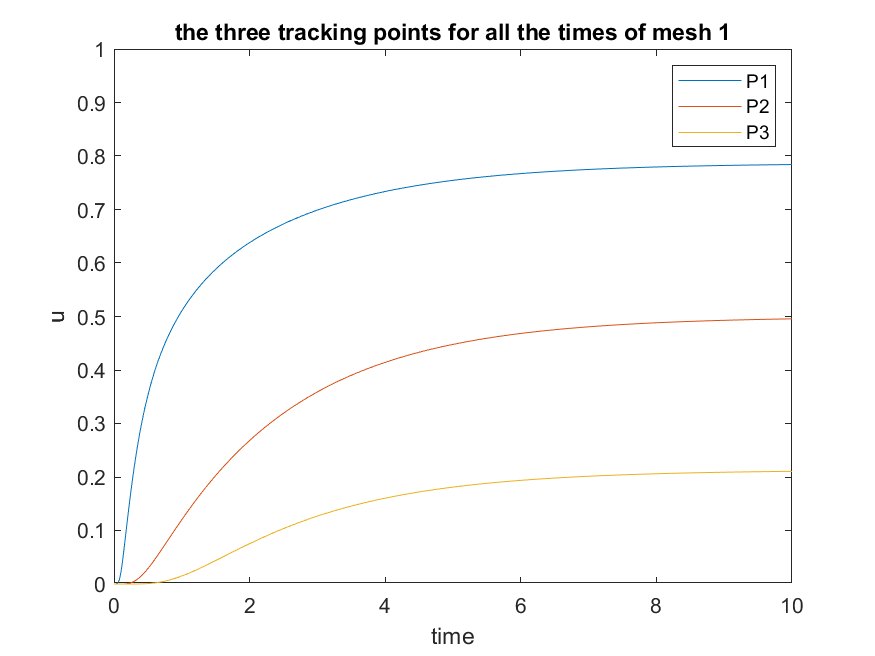
\includegraphics[width=\linewidth,trim=0mm 0mm 0mm 7.5mm, clip]{Images/mesh1/track_chol_mesh1.png}
        \caption{mesh1}
    \end{subfigure}
    \hfill
    \begin{subfigure}{0.45\textwidth}
        \centering
        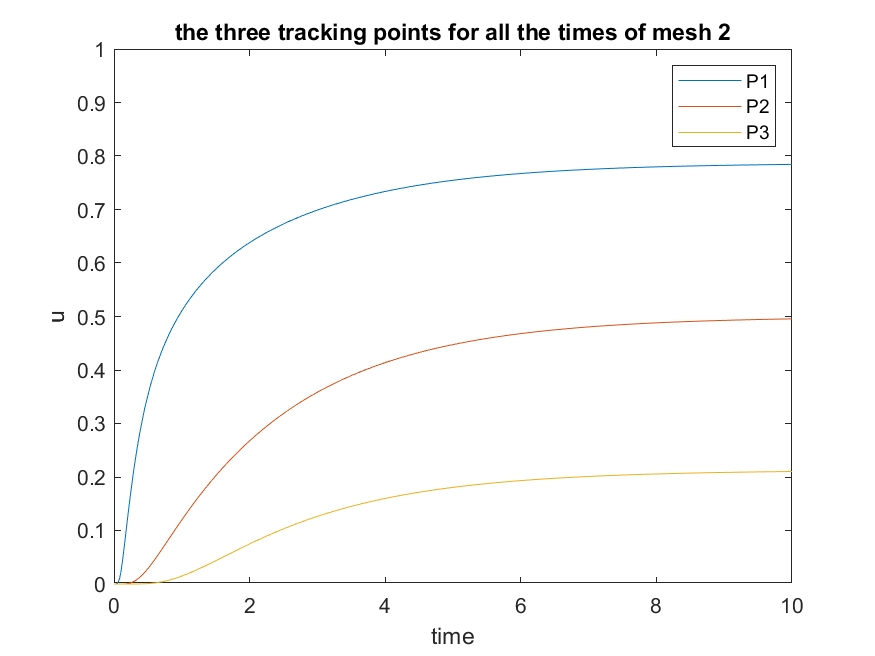
\includegraphics[width=\linewidth,trim=0mm 0mm 0mm 7.5mm, clip]{Images/mesh2/track_chol_mesh2.png}
        \caption{mesh2}
    \end{subfigure}

    \vspace{1em} % Spacing between rows

    \begin{subfigure}{0.45\textwidth}
        \centering
        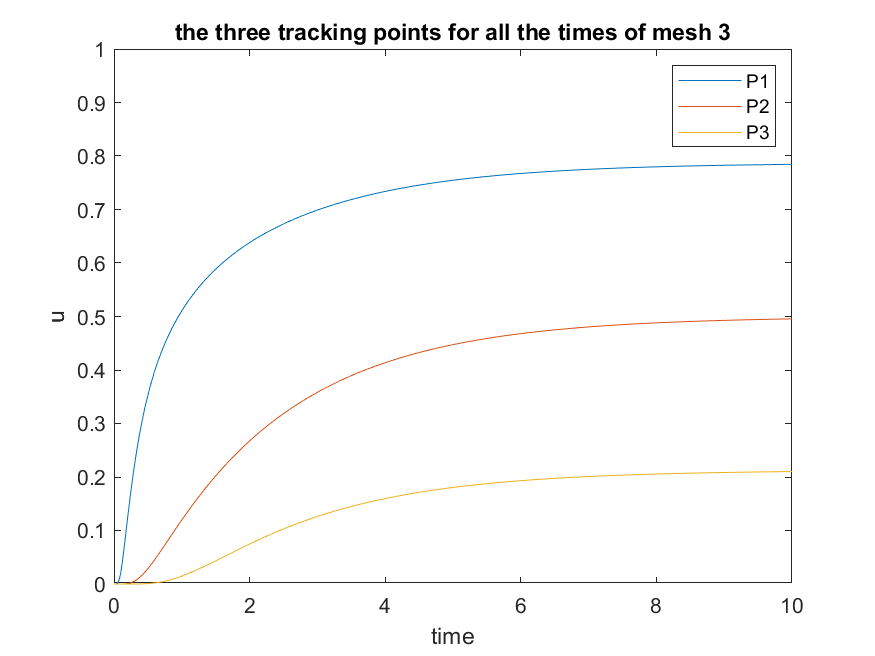
\includegraphics[width=\linewidth,trim=0mm 0mm 0mm 7.5mm, clip]{Images/mesh3/track_chol_mesh3.png}
        \caption{mesh3}
    \end{subfigure}
    \hfill
    \begin{subfigure}{0.45\textwidth}
        \centering
        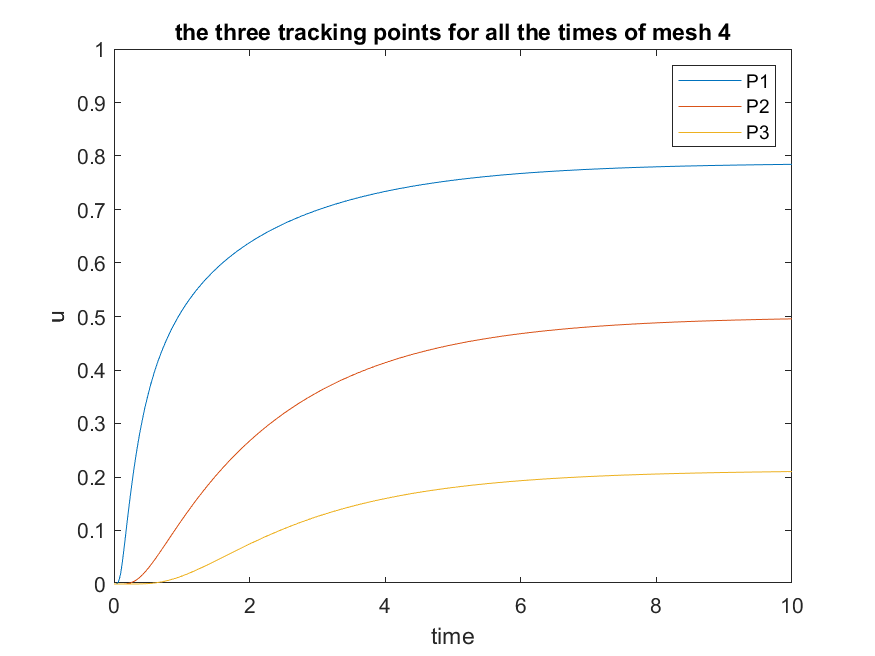
\includegraphics[width=\linewidth,trim=0mm 0mm 0mm 7.5mm, clip]{Images/mesh4/track_chol_mesh4.png}
        \caption{mesh4}
    \end{subfigure}

    \caption{Solution on the three tracking points for all the times and for every meshes}
    \label{fig: track point for all time}
\end{figure}

%---------------------------------------RESIDUAL NORM CHOLENSKY-----------------------------

\begin{figure}[htbp]
    \centering
    \begin{subfigure}{0.45\textwidth}
        \centering
        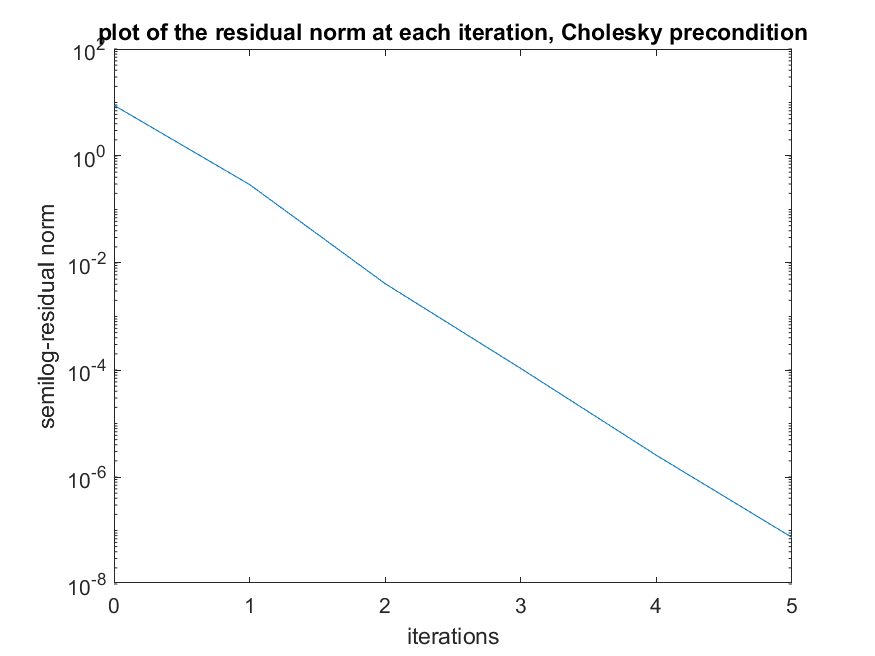
\includegraphics[width=\linewidth,trim=0mm 0mm 0mm 7.5mm, clip]{Images/mesh0/Semilog_Residual_chol_mesh0.png}
        \caption{mesh0}
    \end{subfigure}
    \hfill
    \begin{subfigure}{0.45\textwidth}
        \centering
        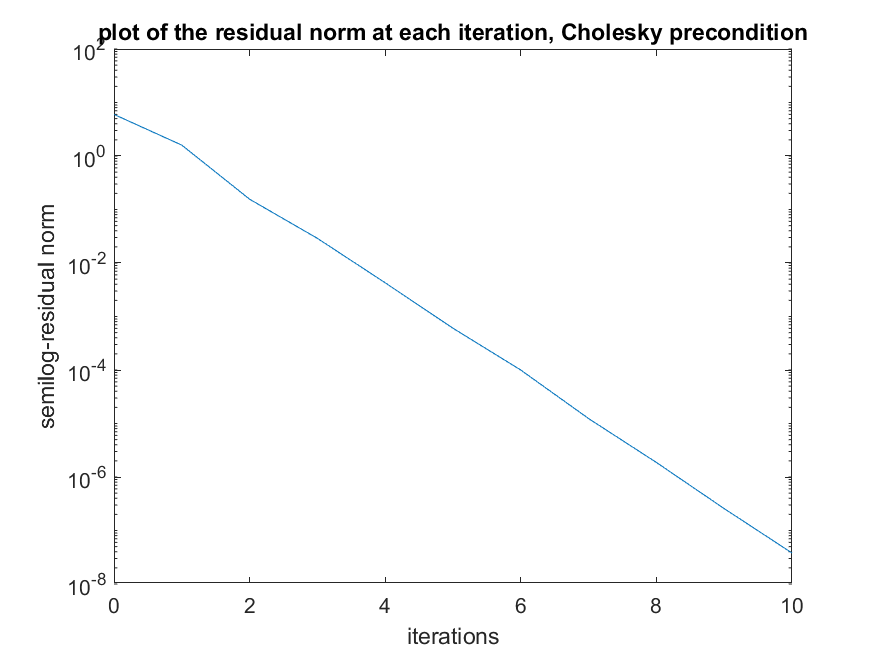
\includegraphics[width=\linewidth,trim=0mm 0mm 0mm 7.5mm, clip]{Images/mesh1/Semilog_Residual_chol_mesh1.png}
        \caption{mesh1}
    \end{subfigure}
    \hfill
    \begin{subfigure}{0.45\textwidth}
        \centering
        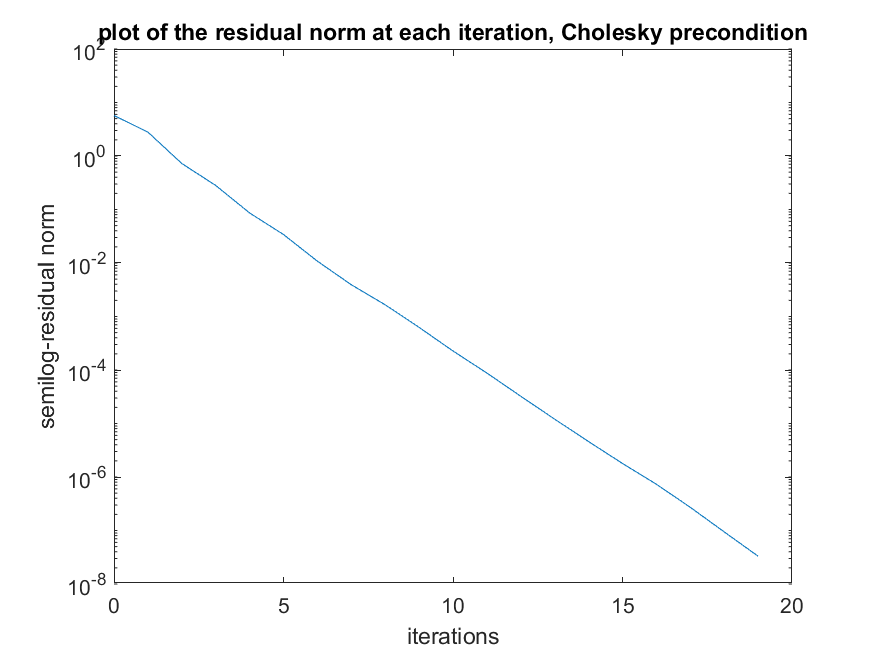
\includegraphics[width=\linewidth,trim=0mm 0mm 0mm 7.5mm, clip]{Images/mesh2/Semilog_Residual_chol_mesh2.png}
        \caption{mesh2}
    \end{subfigure}

    \vspace{1em} % Spacing between rows

    \begin{subfigure}{0.45\textwidth}
        \centering
        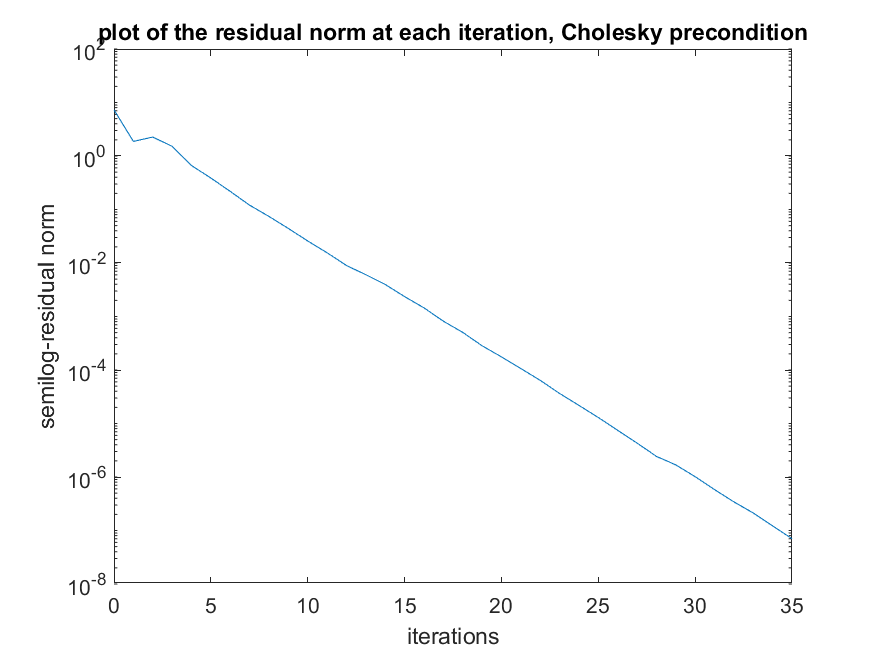
\includegraphics[width=\linewidth,trim=0mm 0mm 0mm 7.5mm, clip]{Images/mesh3/Semilog_Residual_chol_mesh3.png}
        \caption{mesh3}
    \end{subfigure}
    \hfill
    \begin{subfigure}{0.45\textwidth}
        \centering
        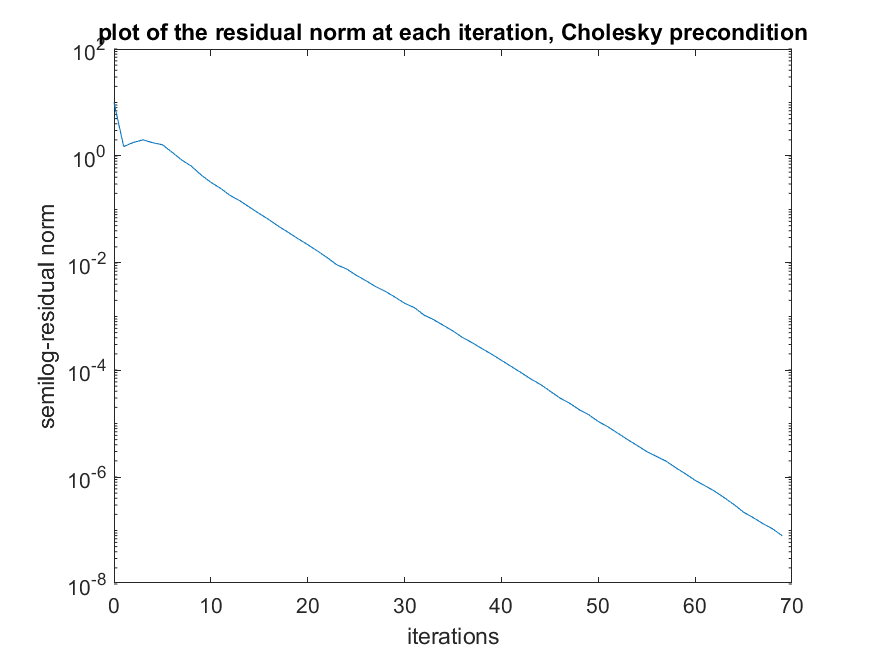
\includegraphics[width=\linewidth,trim=0mm 0mm 0mm 7.5mm, clip]{Images/mesh4/Semilog_Residual_chol_mesh4.png}
        \caption{mesh4}
    \end{subfigure}

    \caption{Value of the Residual norm for the Cholensky Preconditioner in semi-log scale}
    \label{fig: Residual normal cholensky}
\end{figure}

%---------------------------------------RESIDUAL NORM JACOBI-----------------------------

\begin{figure}[htbp]
    \centering
    \begin{subfigure}{0.45\textwidth}
        \centering
        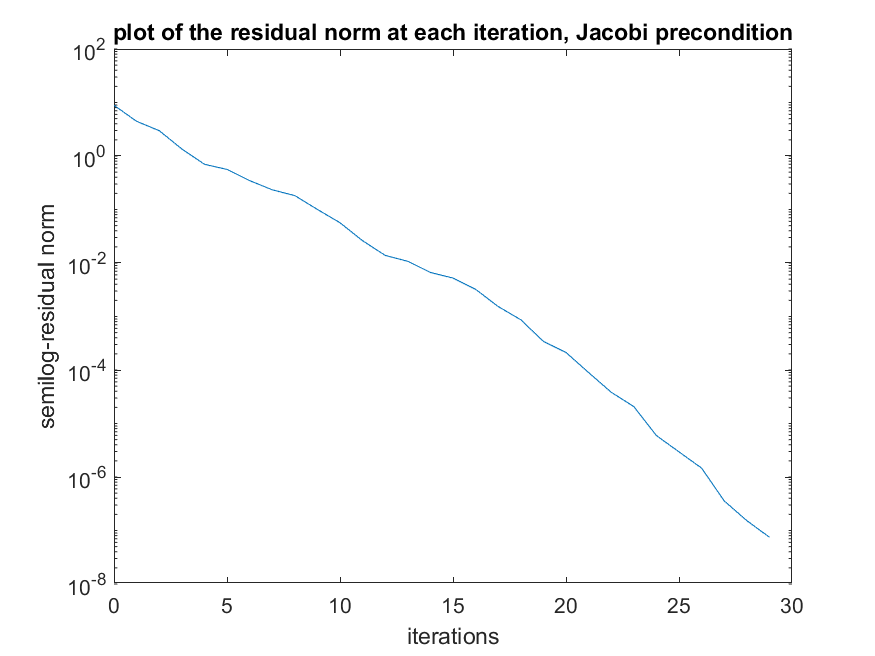
\includegraphics[width=\linewidth,trim=0mm 0mm 0mm 7.5mm, clip]{Images/mesh0/Semilog_Residual_jac_mesh0.png}
        \caption{mesh0}
    \end{subfigure}
    \hfill
    \begin{subfigure}{0.45\textwidth}
        \centering
        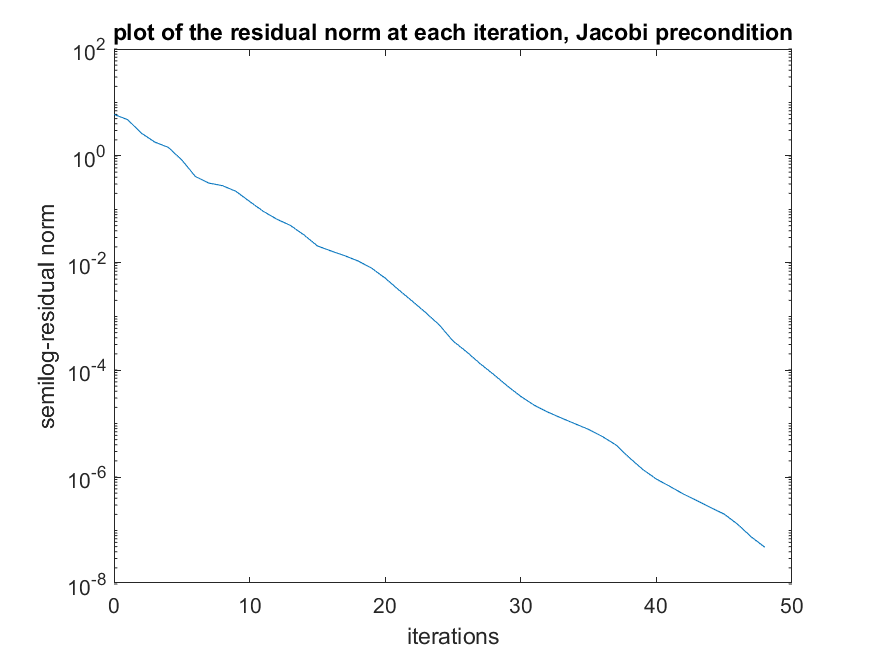
\includegraphics[width=\linewidth,trim=0mm 0mm 0mm 7.5mm, clip]{Images/mesh1/Semilog_Residual_jac_mesh1.png}
        \caption{mesh1}
    \end{subfigure}
    \hfill
    \begin{subfigure}{0.45\textwidth}
        \centering
        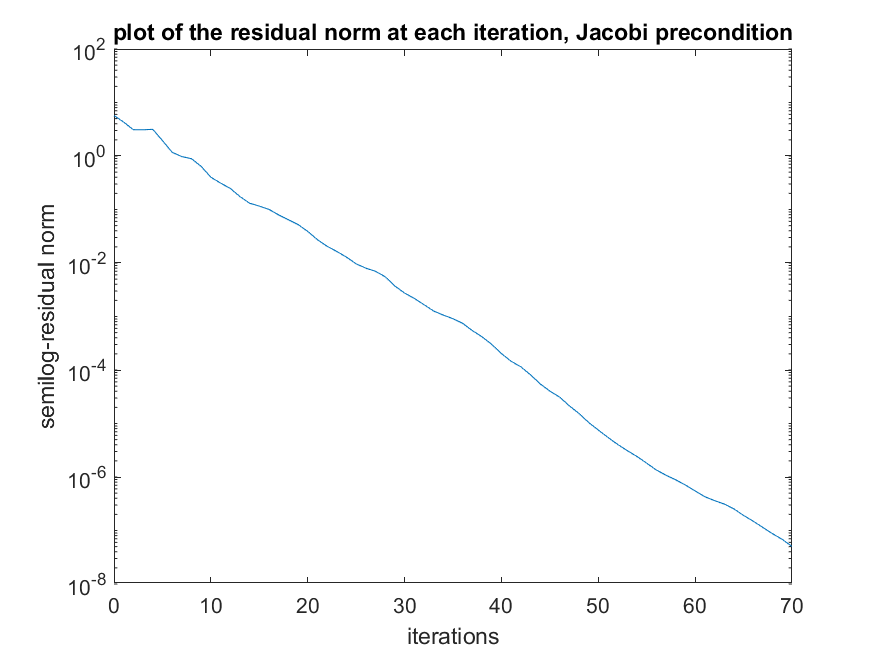
\includegraphics[width=\linewidth,trim=0mm 0mm 0mm 7.5mm, clip]{Images/mesh2/Semilog_Residual_jac_mesh2.png}
        \caption{mesh2}
    \end{subfigure}

    \vspace{1em} % Spacing between rows

    \begin{subfigure}{0.45\textwidth}
        \centering
        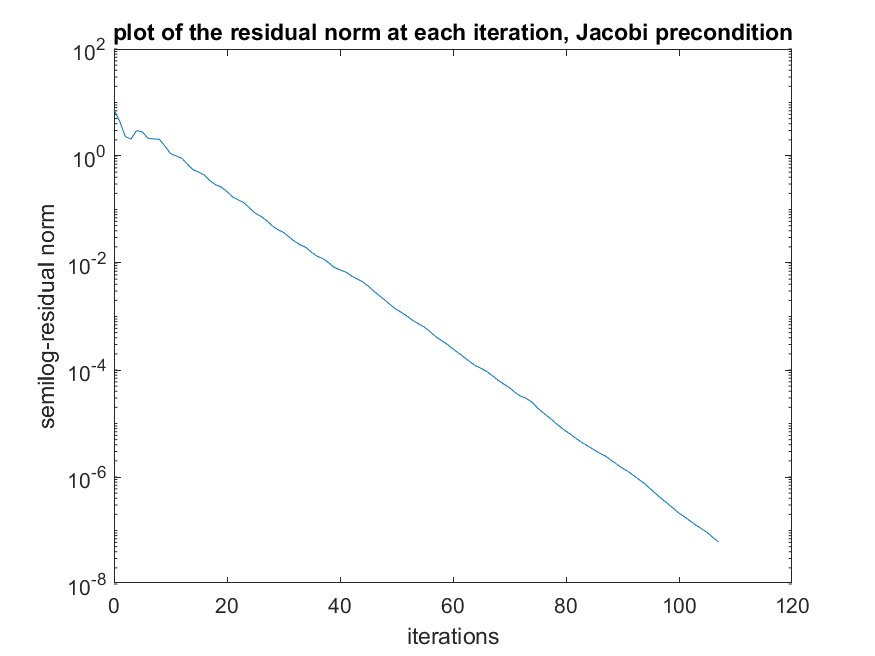
\includegraphics[width=\linewidth,trim=0mm 0mm 0mm 7.5mm, clip]{Images/mesh3/Semilog_Residual_jac_mesh3.png}
        \caption{mesh3}
    \end{subfigure}
    \hfill
    \begin{subfigure}{0.45\textwidth}
        \centering
        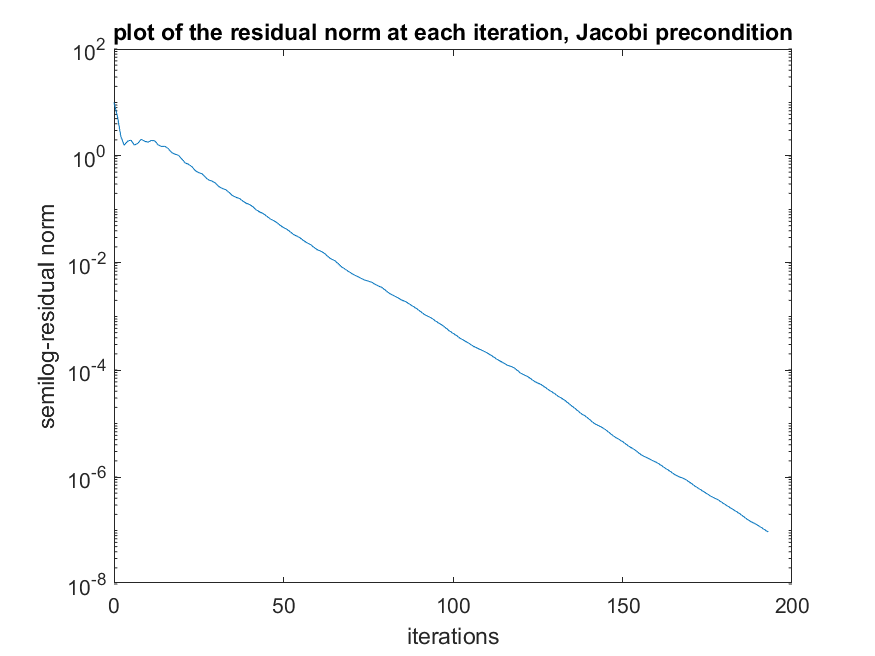
\includegraphics[width=\linewidth,trim=0mm 0mm 0mm 7.5mm, clip]{Images/mesh4/Semilog_Residual_jac_mesh4.png}
        \caption{mesh4}
    \end{subfigure}

    \caption{Value of the Residual norm for the Jacobi Preconditioner in semi-log scale}
    \label{fig: Residual normal jacobi}
\end{figure}

%---------------------------------------TABLE--------------------------------
 
\begin{table}[htbp]
    \centering
    \begin{subtable}{0.45\linewidth}
        \centering
        \begin{tabular}{cccc}
            \hline
            \textbf{Time} & \textbf{P1} & \textbf{P2} & \textbf{P3} \\
            \hline
            2.5 & 0.67116 & 0.31958 & 0.10464 \\
            5   & 0.75329 & 0.44864 & 0.18288 \\
            7.5 & 0.77613 & 0.48538 & 0.2057  \\
            10  & 0.78263 & 0.49584 & 0.2122  \\
            \hline
        \end{tabular}
        \caption{mesh0}
        \label{subtab:mesh0}
    \end{subtable}
    \hfill
    \begin{subtable}{0.45\linewidth}
        \centering
        \begin{tabular}{cccc}
            \hline
            \textbf{Time} & \textbf{P1} & \textbf{P2} & \textbf{P3} \\
            \hline
            2.5 & 0.67183 & 0.31743 & 0.10255 \\
            5   & 0.75419 & 0.44737 & 0.1808 \\
            7.5 & 0.77734 & 0.48481 & 0.20393 \\
            10  & 0.78401 & 0.49561 & 0.2106 \\
            \hline
        \end{tabular}
        \caption{mesh1}
        \label{subtab:mesh1}
    \end{subtable}
    \hfill
    \begin{subtable}{0.45\linewidth}
        \centering
        \begin{tabular}{cccc}
            \hline
            \textbf{Time} & \textbf{P1} & \textbf{P2} & \textbf{P3} \\
            \hline
            2.5 & 0.67183 & 0.3168 & 0.10201 \\
            5   & 0.75428 & 0.44468 & 0.18029 \\
            7.5 & 0.77755 & 0.48465 & 0.20353 \\
            10  & 0.78427 & 0.49554 & 0.2106 \\
            \hline
        \end{tabular}
        \caption{mesh2}
        \label{subtab:mesh2}
    \end{subtable}
    \hfill
    \begin{subtable}{0.45\linewidth}
        \centering
        \begin{tabular}{cccc}
            \hline
            \textbf{Time} & \textbf{P1} & \textbf{P2} & \textbf{P3} \\
            \hline
            2.5 & 0.67185 & 0.31665 & 0.10187 \\
            5   & 0.75433 & 0.4469  & 0.18015 \\
            7.5 & 0.77762 & 0.48462 & 0.20341 \\
            10  & 0.78436 & 0.49555 & 0.21015 \\
            \hline
        \end{tabular}
        \caption{mesh3}
        \label{subtab: mesh3}
    \end{subtable}
    \hfill
    \begin{subtable}{0.45\linewidth}
        \centering
        \begin{tabular}{cccc}
            \hline
            \textbf{Time} & \textbf{P1} & \textbf{P2} & \textbf{P3} \\
            \hline
            2.5 & 0.67184 & 0.31661 & 0.10183 \\
            5   & 0.75433 & 0.44688 & 0.18011 \\
            7.5 & 0.77763 & 0.48461 & 0.20338 \\
            10  & 0.78437 & 0.49554 & 0.21013 \\
            \hline
        \end{tabular}
        \caption{mesh4}
        \label{subtab: mesh4}
    \end{subtable}
    
    \caption{Solution at different times for points $P_1$, $P_2$ and $P_3$ for different meshes}
    \label{tab: data_point}
\end{table}

%---------------------------------------------------

\begin{table}[htbp]
    \centering
    \begin{subtable}{0.45\linewidth}
        \centering
        \begin{tabular}{cccc}
            \hline
            \textbf{Meshes} & \textbf{Iteration} & \textbf{$\varepsilon$} & \textbf{r} \\
            \hline
            0 & 5 & 0.59415 & 0 \\
            1 & 10 & 0.54341 & 1.0934 \\
            2 & 19 & 0.50342 & 1.0794 \\
            3 & 35 & 0.50631 & 0.99429 \\
            4 & 69 & 0.49026 & 1.0327 \\
            \hline
        \end{tabular}
        \caption{Results obtained using Cholesky preconditioner.}
        \label{table:cholesky_results}
    \end{subtable}
    \hfill
    \begin{subtable}{0.45\linewidth}
        \centering
        \begin{tabular}{cccc}
            \hline
            \textbf{Meshes} & \textbf{Iteration} & \textbf{$\varepsilon$} & \textbf{r} \\
            \hline
            0 & 29 & 0.59415 & 0 \\
            1 & 48 & 0.54341 & 1.0934 \\
            2 & 70 & 0.50342 & 1.0794 \\
            3 & 107 & 0.50631 & 0.99429 \\
            4 & 193 & 0.49026 & 1.0327 \\
            \hline
        \end{tabular}
        \caption{Results obtained using Jacobi preconditioner.}
        \label{table:jacobi_results}
    \end{subtable}
    \caption{value of iteration, error $\varepsilon$ the ratio r for every meshes}
    \label{tab: table_R_error}
\end{table}

 % Section/Chapter entries can be done in the Main.tex file or in a  
                       % separate tex file for longer and more complex documents





\end{document}
%  -------------------------------------------------
%  --------- The document ends from here ----------- 
%  -------------------------------------------------
